\subsection{Enumeratoren}



Enumeratoren sind für die Erforschung eines Surchraums verantwortlich. Sie generieren basierend auf einer Anfrage unterschiedliche alternative Pläne. Es lässt sich im Allgemeinen zwischen zwei Klassen von Enumeratoren unterscheiden: dynamisch programmierte und regelbasierte Enumeratoren.  \todo{Quelle}

Das Konzept der dynamischen Programmierung wurde zuerst durch IBM's System R umgesetzt \cite{selinger1979access}. In diesem System wird die Reihenfolge der JOINs, die für eine Anfrage notwendig sind verändert, um die Anfrage zu optimieren. Der Search Space, der durch den Enumerator erforscht wird, besteht aus Join Trees. Je nach Enumerator werden nur bestimmte Join Trees behandelt.


\begin{figure}[h]
  \centering
  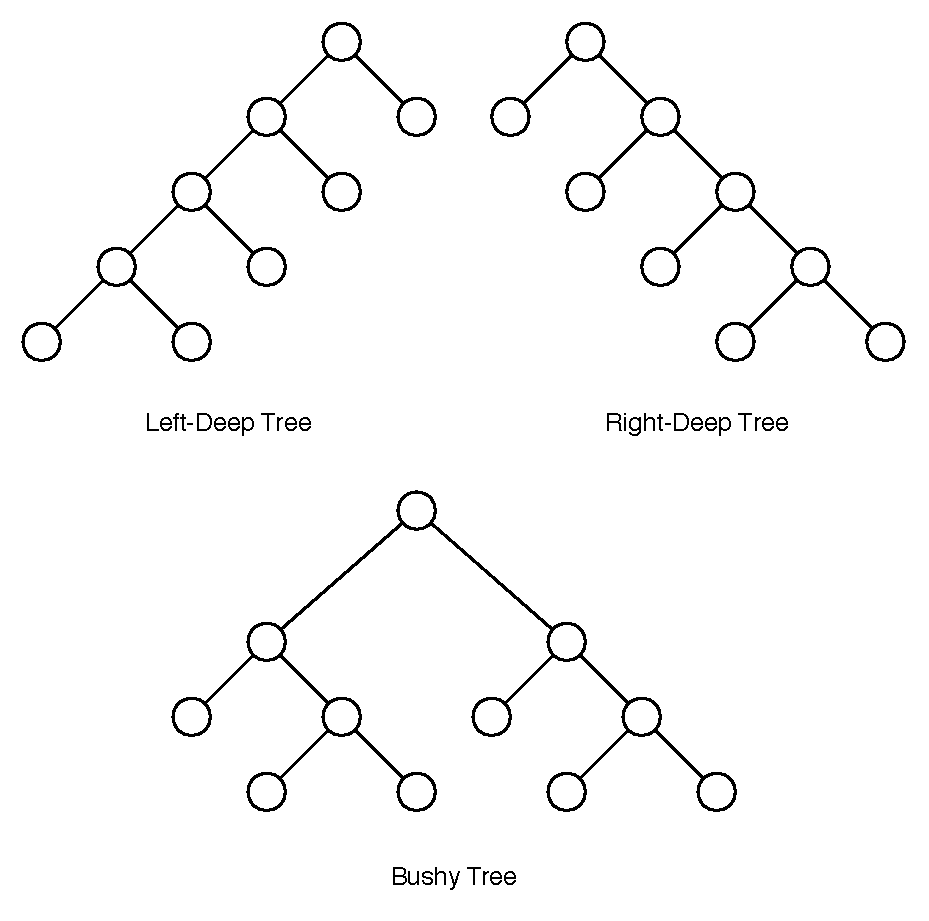
\includegraphics[width=\textwidth]{02_Related_Work/TreeTypes.pdf}
  \caption{Tree Types}
  \label{TreeTypes}
\end{figure}

Je nach \ac{DBMS} kann sich ein Enumerator nur auf einen Teil des gesamten Search Spaces beschränken. So ist es möglich, dass eine Beschränkung auf Grund der Form eines Baumes gebildet wird. Grob lässt sich wie in Abb. \ref{TreeTypes} zu sehen ist, zwischen drei Arten von Bäumen unterscheiden, Left-Deep, Bushy und Right-Deep Trees. Je nach behandelter Join Art werden mehr oder weniger potenzielle Bäume aus dem Suchraum ausgeschlossen. Je nach Größe des potenziellen Suchraums kann sich die Suche effizienter oder weniger effizient gestalten. Einige \ac{DBMS} Hersteller argumentieren \todo{QUELLE}, dass die Beschränkung auf beispielsweise Left-Deep Trees vorteilhaft wäre, da Aufwand für die Suche nach den Plänen gespart werden kann und trotzdem eine große Menge an alternativen Plänen erzeugt wird, die für sich genommen auch einen Plan nahe dem optimalen Plan enthält. 